\documentclass{beamer}
\mode<presentation>
\usepackage{amsmath,amssymb,mathtools}
\usepackage{textcomp}
\usepackage{listings}
\usepackage{url}
\usepackage{graphicx}
\usepackage{booktabs}
\def\UrlBreaks{\do\/\do-}
\usetheme{Boadilla}
\usecolortheme{lily}
\setbeamertemplate{footline}{
  \leavevmode%
  \hbox{%
  \begin{beamercolorbox}[wd=\paperwidth,ht=2ex,dp=1ex,right]{author in head/foot}%
    \insertframenumber{} / \inserttotalframenumber\hspace*{2ex}
  \end{beamercolorbox}}%
  \vskip0pt%
}
\setbeamertemplate{navigation symbols}{}
\lstset{
  frame=single,
  breaklines=true,
  columns=fullflexible,
  basicstyle=\ttfamily\tiny
}
\numberwithin{equation}{section}
\providecommand{\nCr}[2]{\,^{#1}C_{#2}}
\providecommand{\nPr}[2]{\,^{#1}P_{#2}}
\providecommand{\mbf}{\mathbf}
\providecommand{\pr}[1]{\ensuremath{\Pr\left(#1\right)}}
\providecommand{\qfunc}[1]{\ensuremath{Q\left(#1\right)}}
\providecommand{\sbrak}[1]{\ensuremath{{}\left[#1\right]}}
\providecommand{\lsbrak}[1]{\ensuremath{{}\left[#1\right.}}
\providecommand{\rsbrak}[1]{\ensuremath{\left.#1\right]}}
\providecommand{\brak}[1]{\ensuremath{\left(#1\right)}}
\providecommand{\lbrak}[1]{\ensuremath{\left(#1\right.}}
\providecommand{\rbrak}[1]{\ensuremath{\left.#1\right)}}
\providecommand{\cbrak}[1]{\ensuremath{\left\{#1\right\}}}
\providecommand{\lcbrak}[1]{\ensuremath{\left\{#1\right.}}
\providecommand{\rcbrak}[1]{\ensuremath{\left.#1\right\}}}
\theoremstyle{remark}
\newtheorem{rem}{Remark}
\newcommand{\sgn}{\mathop{\mathrm{sgn}}}
\providecommand{\abs}[1]{\left\vert#1\right\vert}
\providecommand{\res}[1]{\Res\displaylimits_{#1}}
\providecommand{\norm}[1]{\lVert#1\rVert}
\providecommand{\mtx}[1]{\mathbf{#1}}
\providecommand{\mean}[1]{E\left[ #1 \right]}
\providecommand{\fourier}{\overset{\mathcal{F}}{ \rightleftharpoons}}
\providecommand{\system}{\overset{\mathcal{H}}{ \longleftharpoons}}
\providecommand{\dec}[2]{\ensuremath{\overset{#1}{\underset{#2}{\gtrless}}}}
\newcommand{\myvec}[1]{\ensuremath{\begin{pmatrix}#1\end{pmatrix}}}
\newcommand{\mydet}[1]{\ensuremath{\begin{vmatrix}#1\end{vmatrix}}}
\let\vec\mathbf

\title{ODE -- Problem 1.2.70}
\author{ee25btech11056 -- Suraj.N}

\begin{document}

%-------------------------------------------------------------
\begin{frame}
  \titlepage
\end{frame}

%-------------------------------------------------------------
\begin{frame}{Problem Statement}

\textbf{Problem 1.2.70}

The solution of the ordinary differential equation
\[
  \frac{dy}{dx} = x^2 + 2y
\]
is:

\begin{enumerate}
  \item $y = \dfrac{2}{3}x^2 + 4x$
  \item $y = \sqrt{\dfrac{2}{3}x^2 + 4x + k}$
  \item $y = \dfrac{2}{3}x^3 - 4x + k$
  \item $y = \dfrac{2}{3}x^3 + 4x + k$
\end{enumerate}

\end{frame}

%-------------------------------------------------------------
\begin{frame}{Identifying the ODE Type}

The equation is:
\[
  \frac{dy}{dx} - 2y = x^2
\]

This is a \textbf{first-order linear ODE} of the standard form:
\[
  \frac{dy}{dx} + P(x)\,y = Q(x)
\]

with $P(x) = -2$ and $Q(x) = x^2$.

The method of solution is the \textbf{integrating factor method}.

\begin{enumerate}
  \item Find the integrating factor $\mu(x) = e^{\int P(x)\,dx}$
  \item Multiply both sides by $\mu(x)$
  \item Recognise the left side as $\dfrac{d}{dx}[\mu(x)\,y]$
  \item Integrate both sides and solve for $y$
\end{enumerate}

\end{frame}

%-------------------------------------------------------------
\begin{frame}{Step 1: Integrating Factor}

The integrating factor is:
\[
  \mu(x) = e^{\int P(x)\,dx} = e^{\int (-2)\,dx} = e^{-2x}
\]

Multiply both sides of the ODE by $e^{-2x}$:
\[
  e^{-2x}\frac{dy}{dx} - 2e^{-2x}y = x^2 e^{-2x}
\]

The left side is the exact derivative of $e^{-2x}y$:
\[
  \frac{d}{dx}\!\left[e^{-2x}y\right] = x^2 e^{-2x}
\]

This works because by the product rule:
\[
  \frac{d}{dx}\!\left[e^{-2x}y\right]
  = e^{-2x}\frac{dy}{dx} + (-2)e^{-2x}y
  = e^{-2x}\frac{dy}{dx} - 2e^{-2x}y
\]

which matches the left side exactly.

\end{frame}

%-------------------------------------------------------------
\begin{frame}{Step 2: Integrating Both Sides}

Integrate both sides with respect to $x$:
\[
  e^{-2x}y = \int x^2 e^{-2x}\,dx
\]

Evaluate $\int x^2 e^{-2x}\,dx$ using integration by parts twice.

Let $I = \int x^2 e^{-2x}\,dx$.

\textbf{First integration by parts:} $u = x^2$, $dv = e^{-2x}dx$
\[
  I = -\frac{x^2}{2}e^{-2x} + \int x\,e^{-2x}\,dx
\]

\textbf{Second integration by parts:} $u = x$, $dv = e^{-2x}dx$
\[
  \int x\,e^{-2x}\,dx = -\frac{x}{2}e^{-2x} + \int \frac{1}{2}e^{-2x}\,dx
  = -\frac{x}{2}e^{-2x} - \frac{1}{4}e^{-2x}
\]

Combining:
\[
  I = -\frac{x^2}{2}e^{-2x} - \frac{x}{2}e^{-2x} - \frac{1}{4}e^{-2x} + C
\]

\end{frame}

%-------------------------------------------------------------
\begin{frame}{Step 3: Solving for $y$}

Substituting back:
\[
  e^{-2x}y
  = -\frac{x^2}{2}e^{-2x} - \frac{x}{2}e^{-2x} - \frac{1}{4}e^{-2x} + C
\]

Divide every term by $e^{-2x}$ (i.e.\ multiply by $e^{2x}$):
\[
  y = -\frac{x^2}{2} - \frac{x}{2} - \frac{1}{4} + C e^{2x}
\]

The general solution is:
\[
  \boxed{y = -\frac{x^2}{2} - \frac{x}{2} - \frac{1}{4} + C e^{2x}}
\]

where $C$ is an arbitrary constant.

\end{frame}

%-------------------------------------------------------------

%-------------------------------------------------------------
\begin{frame}{Correct Answer}

The exact general solution from the integrating factor method is:
\[
  \boxed{y = Ce^{2x} - \frac{x^2}{2} - \frac{x}{2} - \frac{1}{4}}
\]

This is the complete and correct answer. None of the polynomial options
exactly match since they omit the $e^{2x}$ term.

\end{frame}

%-------------------------------------------------------------
\begin{frame}{Laplace Transform Solution -- Setup}

Take the Laplace transform of both sides of $\dfrac{dy}{dx} - 2y = x^2$.

Recall the key Laplace transform properties:
\begin{enumerate}
  \item $\mathcal{L}\!\left\{\dfrac{dy}{dx}\right\} = sY(s) - y(0)$
  \item $\mathcal{L}\{y\} = Y(s)$
  \item $\mathcal{L}\{x^2\} = \dfrac{2}{s^3}$
\end{enumerate}

Applying $\mathcal{L}\{\cdot\}$ to both sides:
\[
  \mathcal{L}\!\left\{\frac{dy}{dx}\right\} - 2\,\mathcal{L}\{y\} = \mathcal{L}\{x^2\}
\]
\[
  sY(s) - y(0) - 2Y(s) = \frac{2}{s^3}
\]

Let the initial condition be $y(0) = y_0$ (arbitrary constant).

\end{frame}

%-------------------------------------------------------------
\begin{frame}{Laplace Transform Solution -- Solving for $Y(s)$}

Collect terms in $Y(s)$:
\[
  (s - 2)\,Y(s) = \frac{2}{s^3} + y_0
\]

Solve for $Y(s)$:
\[
  Y(s) = \frac{2}{s^3(s-2)} + \frac{y_0}{s-2}
\]

Apply partial fractions to $\dfrac{2}{s^3(s-2)}$:
\[
  \frac{2}{s^3(s-2)}
  = \frac{A}{s} + \frac{B}{s^2} + \frac{D}{s^3} + \frac{E}{s-2}
\]

Multiplying both sides by $s^3(s-2)$ and matching coefficients:
\[
  2 = As^2(s-2) + Bs(s-2) + D(s-2) + Es^3
\]

Setting $s=0$: $\;2 = D(-2) \Rightarrow D = -1$

Setting $s=2$: $\;2 = E(8) \Rightarrow E = \frac{1}{4}$

\end{frame}

%-------------------------------------------------------------
\begin{frame}{Laplace Transform -- Partial Fractions Completed}

Expanding and matching $s^3$, $s^2$, $s^1$ coefficients:

From $s^3$: $\;0 = A + E \Rightarrow A = -E = -\dfrac{1}{4}$

From $s^2$: $\;0 = -2A + B \Rightarrow B = 2A = -\dfrac{1}{2}$

So:
\[
  \frac{2}{s^3(s-2)}
  = \frac{-1/4}{s} + \frac{-1/2}{s^2} + \frac{-1}{s^3} + \frac{1/4}{s-2}
\]

Therefore:
\[
  Y(s) = -\frac{1}{4s} - \frac{1}{2s^2} - \frac{1}{s^3}
         + \frac{1/4}{s-2} + \frac{y_0}{s-2}
\]
\[
  Y(s) = -\frac{1}{4s} - \frac{1}{2s^2} - \frac{1}{s^3}
         + \frac{y_0 + 1/4}{s-2}
\]

\end{frame}

%-------------------------------------------------------------
\begin{frame}{Laplace Transform -- Inverse Transform}

Apply the inverse Laplace transform using:
\begin{enumerate}
  \item $\mathcal{L}^{-1}\!\left\{\dfrac{1}{s}\right\} = 1$
  \item $\mathcal{L}^{-1}\!\left\{\dfrac{1}{s^2}\right\} = x$
  \item $\mathcal{L}^{-1}\!\left\{\dfrac{1}{s^3}\right\} = \dfrac{x^2}{2}$
  \item $\mathcal{L}^{-1}\!\left\{\dfrac{1}{s-2}\right\} = e^{2x}$
\end{enumerate}

Taking $\mathcal{L}^{-1}\{Y(s)\}$:
\[
  y(x) = -\frac{1}{4} - \frac{x}{2} - \frac{x^2}{2}
         + \!\left(y_0 + \frac{1}{4}\right)e^{2x}
\]

Let $C = y_0 + \dfrac{1}{4}$ (absorbed into the arbitrary constant). Then:
\[
  \boxed{y(x) = Ce^{2x} - \frac{x^2}{2} - \frac{x}{2} - \frac{1}{4}}
\]

This is \textbf{identical} to the result from the integrating factor method,
confirming the solution is correct.

\end{frame}
\begin{frame}{Plot} 

\begin{figure}[h!]
  \centering
  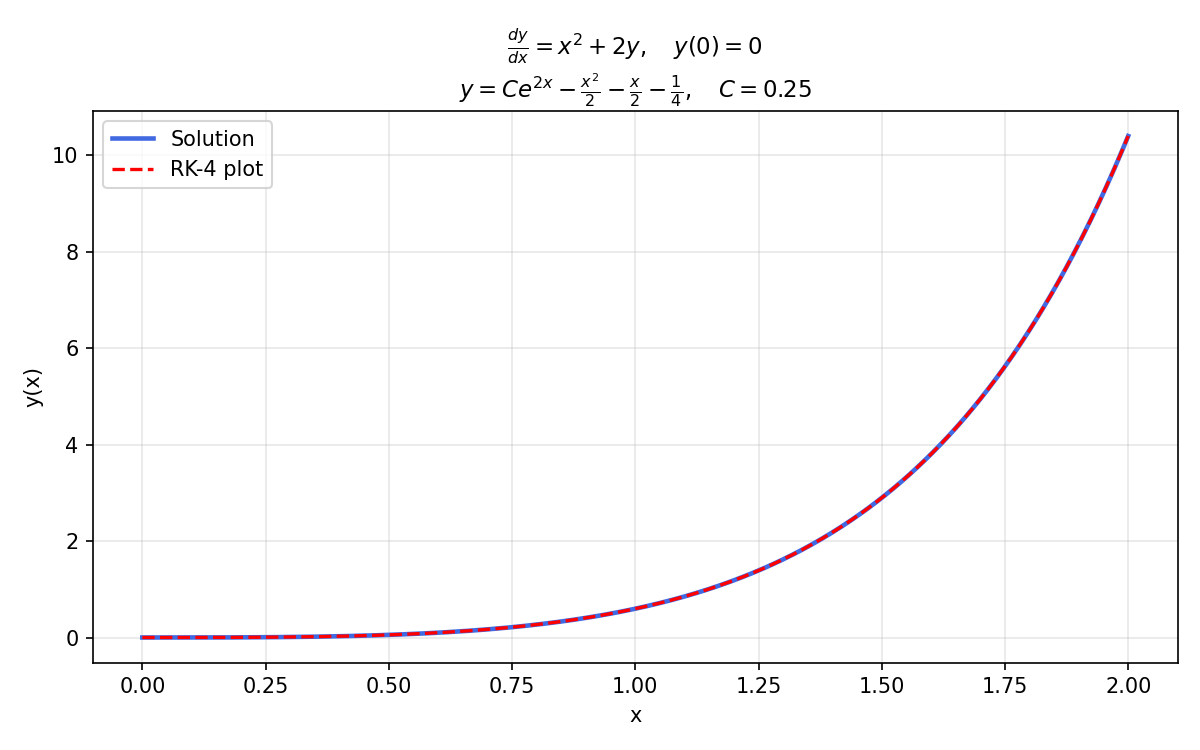
\includegraphics[width=0.9\columnwidth]{figs/rk4_plot.png} 
  \caption{Plot}
  \label{Fig1}
\end{figure}


\end{frame} 

\end{frame}
\begin{frame}{Plot-Comparison} 

\begin{figure}[h!]
  \centering
  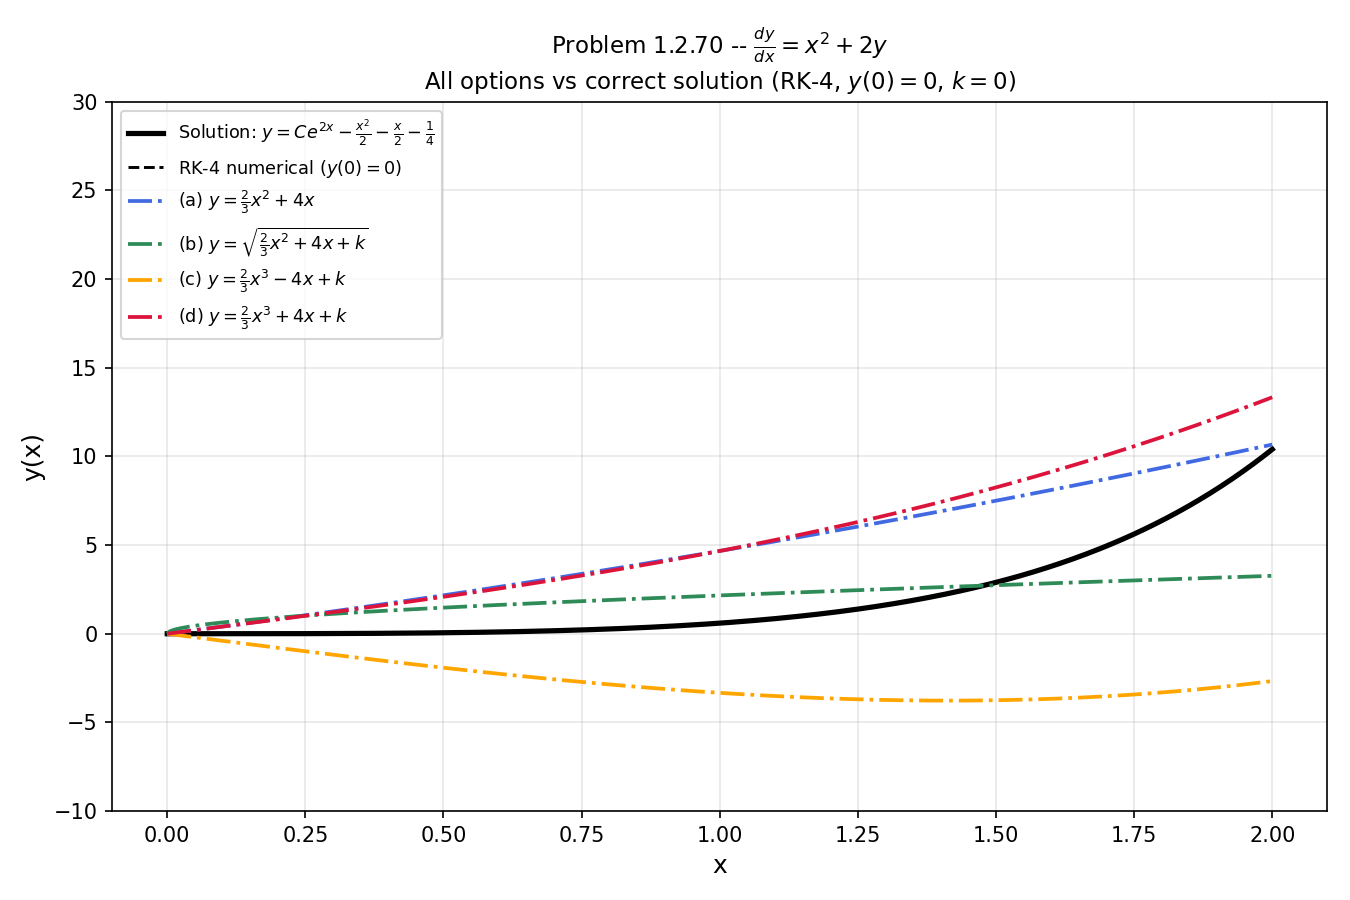
\includegraphics[width=0.9\columnwidth]{figs/rk4_options.png} 
  \caption{Plot}
  \label{Fig1}
\end{figure}


\end{frame} 

\begin{frame}[fragile]{Python Code: RK-4 Plots}

\lstset{basicstyle=\ttfamily\scriptsize}
\begin{lstlisting}[language=Python]
import numpy as np
import matplotlib.pyplot as plt
from scipy.integrate import solve_ivp

# ODE: dy/dx = x^2 + 2y
def f(x, y):
    return x**2 + 2*y

# Exact general solution: y = C*exp(2x) - x^2/2 - x/2 - 1/4
# With y(0) = 0 => C = 0.25
def exact(x):
    return 0.25 * np.exp(2*x) - x**2/2 - x/2 - 0.25

x_eval = np.linspace(0.0, 2.0, 500)

# RK-4 solution (y(0) = 0)
sol = solve_ivp(f, (0.0, 2.0), [0.0], method='RK45',
                t_eval=x_eval, rtol=1e-8, atol=1e-10)

# Option functions (k=0 chosen for plotting)
k = 0
opt_a = (2/3)*x_eval**2 + 4*x_eval
opt_b = np.sqrt(np.abs((2/3)*x_eval**2 + 4*x_eval + k))
opt_c = (2/3)*x_eval**3 - 4*x_eval + k
opt_d = (2/3)*x_eval**3 + 4*x_eval + k
\end{lstlisting} 
\end{frame}


%-------------------------------------------------------------
\begin{frame}[fragile]{Python Code: RK-4 Solution and Plot}

\lstset{basicstyle=\ttfamily\scriptsize}
\begin{lstlisting}[language=Python]
plt.figure(figsize=(9, 6))

plt.plot(x_eval, exact(x_eval),  'k',   lw=2.5, label=r'Solution: $y=Ce^{2x}-\frac{x^2}{2}-\frac{x}{2}-\frac{1}{4}$')
plt.plot(sol.t,  sol.y[0],       'k--', lw=1.4, label='RK-4 numerical ($y(0)=0$)')
plt.plot(x_eval, opt_a, 'royalblue',  lw=1.8, ls='-.',  label=r'(a) $y=\frac{2}{3}x^2+4x$')
plt.plot(x_eval, opt_b, 'seagreen',   lw=1.8, ls='-.',  label=r'(b) $y=\sqrt{\frac{2}{3}x^2+4x+k}$')
plt.plot(x_eval, opt_c, 'orange',     lw=1.8, ls='-.',  label=r'(c) $y=\frac{2}{3}x^3-4x+k$')
plt.plot(x_eval, opt_d, 'crimson',    lw=1.8, ls='-.',  label=r'(d) $y=\frac{2}{3}x^3+4x+k$')

plt.xlabel('x', fontsize=12)
plt.ylabel('y(x)', fontsize=12)
plt.title(r'Problem 1.2.70 -- $\frac{dy}{dx} = x^2 + 2y$'
          '\nAll options vs correct solution (RK-4, $y(0)=0$, $k=0$)',
          fontsize=11)
plt.legend(fontsize=8.5, loc='upper left')
plt.ylim(-10, 30)
plt.grid(alpha=0.3)
plt.tight_layout()
plt.savefig('rk4_options.png', dpi=150)
plt.show()
\end{lstlisting} 
\end{frame}


%-------------------------------------------------------------
\begin{frame}[fragile]{Python Code: RK-4 Solution and Plot}

\lstset{basicstyle=\ttfamily\scriptsize}
\begin{lstlisting}[language=Python]
import numpy as np
import matplotlib.pyplot as plt
from scipy.integrate import solve_ivp

def f(x, y):
    return x**2 + 2*y

def exact(x, C):
    return C * np.exp(2*x) - x**2/2 - x/2 - 0.25

x0, y0 = 0.0, 0.0
C = y0 + 0.25

x_span = (0.0, 2.0)
x_eval = np.linspace(0.0, 2.0, 500)

sol   = solve_ivp(f, x_span, [y0], method='RK45',
                  t_eval=x_eval, rtol=1e-8, atol=1e-10)
y_ex  = exact(x_eval, C)

plt.figure(figsize=(8, 5))
plt.plot(x_eval, y_ex,   'royalblue', lw=2.2, label='Solution')
plt.plot(sol.t,  sol.y[0], 'r--',    lw=1.6, label='RK-4 plot')
plt.xlabel('x'); plt.ylabel('y(x)')
plt.title(r"$\frac{dy}{dx} = x^2 + 2y,\quad y(0)=0$"
          "\n"
          r"$y = Ce^{2x} - \frac{x^2}{2} - \frac{x}{2} - \frac{1}{4},\quad C = 0.25$",
          fontsize=11)
plt.legend(fontsize=10)
plt.grid(alpha=0.3)
plt.tight_layout()
plt.savefig('rk4_plot.png', dpi=150)
plt.show()
\end{lstlisting}

\end{frame}

%-------------------------------------------------------------
\begin{frame}[fragile]{Python Code: Verification}

\lstset{basicstyle=\ttfamily\scriptsize}
\begin{lstlisting}[language=Python]
import sympy as sp

x = sp.Symbol('x')
C = sp.Symbol('C')

# General solution
y = C*sp.exp(2*x) - x**2/2 - x/2 - sp.Rational(1,4)

# Compute dy/dx
dydx = sp.diff(y, x)

# Check dy/dx - 2y == x^2
residual = sp.simplify(dydx - 2*y - x**2)
print("Residual (should be 0):", residual)

# Verify option (c): y = (2/3)x^3 - 4x + k
k = sp.Symbol('k')
y_c = sp.Rational(2,3)*x**3 - 4*x + k
dydx_c = sp.diff(y_c, x)
res_c = sp.simplify(dydx_c - 2*y_c - x**2)
print("Option (c) residual:", res_c)
\end{lstlisting}

\end{frame}

%-------------------------------------------------------------
\begin{frame}[fragile]{Python Code: Verification}

\lstset{basicstyle=\ttfamily\scriptsize}
\begin{lstlisting}[language=Python]

# Verify option (d): y = (2/3)x^3 + 4x + k
y_d = sp.Rational(2,3)*x**3 + 4*x + k
dydx_d = sp.diff(y_d, x)
res_d = sp.simplify(dydx_d - 2*y_d - x**2)
print("Option (d) residual:", res_d)

print("\nExact general solution:")
print("y =", y)
\end{lstlisting}

\end{frame}

%-------------------------------------------------------------
\begin{frame}{Conclusion}

The ODE $\dfrac{dy}{dx} = x^2 + 2y$ is solved as follows:

\begin{enumerate}
  \item Rewrite as $\dfrac{dy}{dx} - 2y = x^2$ (linear ODE, $P=-2$, $Q=x^2$)
  \item Integrating factor: $\mu = e^{-2x}$
  \item Multiply through and integrate using integration by parts twice
  \item Solve for $y$:
        \[
          y = Ce^{2x} - \frac{x^2}{2} - \frac{x}{2} - \frac{1}{4}
        \]
  \item The Laplace transform method gives the same result
  \item RK-4 numerical solution confirms the exact solution
  \item SymPy symbolic verification confirms the residual is zero
\end{enumerate}

None of the four given options (a)--(d) exactly match the general solution
because they omit the $Ce^{2x}$ homogeneous term. The general solution is:
\[
  \boxed{y = Ce^{2x} - \frac{x^2}{2} - \frac{x}{2} - \frac{1}{4}}
\]

\end{frame}

\end{document}
